\section{What models and what signals?}
Modern physics involves a constant iteration between theoretical model-building, new data collection, and the attempted falsification of models with that data. This thesis is concerned with pulsar glitches, solar flares, and continuously-emitted gravitational waves from neutron stars in accreting binary systems. While these topics are disparate, there is overlap in the methodology with which specific, bespoke statistical models are built to test and explore the underlying physics. 

The connections are outlined diagrammatically in Figure~\ref{fig:thesis_schema}. Rapidly-rotating neutron stars are often seen as pulsars, with remarkably regular pulsed radio emission. These radio pulsations are timed using phase-connected models. The predictable spin of some pulsars is sporadically interrupted by timing irregularities known as ``glitches''. These glitches are suspected to arise from the sudden relaxation of steadily-built-up stress in the interior. An analogous phenomenon of stress build-up and release is believed to drive solar flares. Stress-relax models are falsifiable using long-term statistics calculated from the observed sequences of waiting times between and sizes of events. The spin of neutron stars in binary systems is modulated due to accretion from a companion star, and possibly gravitational wave emission if such accretion builds a time-varying mass quadrupole. Precision timing using pulsations observed in the X-ray emission from the neutron star in these systems enables highly-sensitive searches for continuous gravitational waves. 

The remainder of this chapter serves as an introduction and literature review of the underlying theoretical physics and observational evidence of the above phenomena. In Section~\ref{sec:intro_ns} we present a taxonomical overview of neutron stars from an observational perspective. In Section~\ref{sec:intro_timing} we discuss pulsar timing and glitch detection. In Section~\ref{sec:intro_struc} we review what is known about the structure of neutron stars. In Section~\ref{sec:intro_glitch} we discuss the phenomenology and statistics of glitches, and how they are triggered. We shift focus to general statistical models built to understand complex systems, including solar flares, which undergo stress-accumulation and release in Section~\ref{sec:intro_stress}. In Section~\ref{sec:intro_cw} we introduce gravitational wave emission in general, the specific case of continuous gravitational waves, and discuss accreting millisecond X-ray pulsars (AMXPs) as potential continuous gravitational waves sources. Finally, we provide an outline for the structure of the remainder of the thesis in Section~\ref{sec:intro_outline}.

\begin{figure}[t]
    \centering
    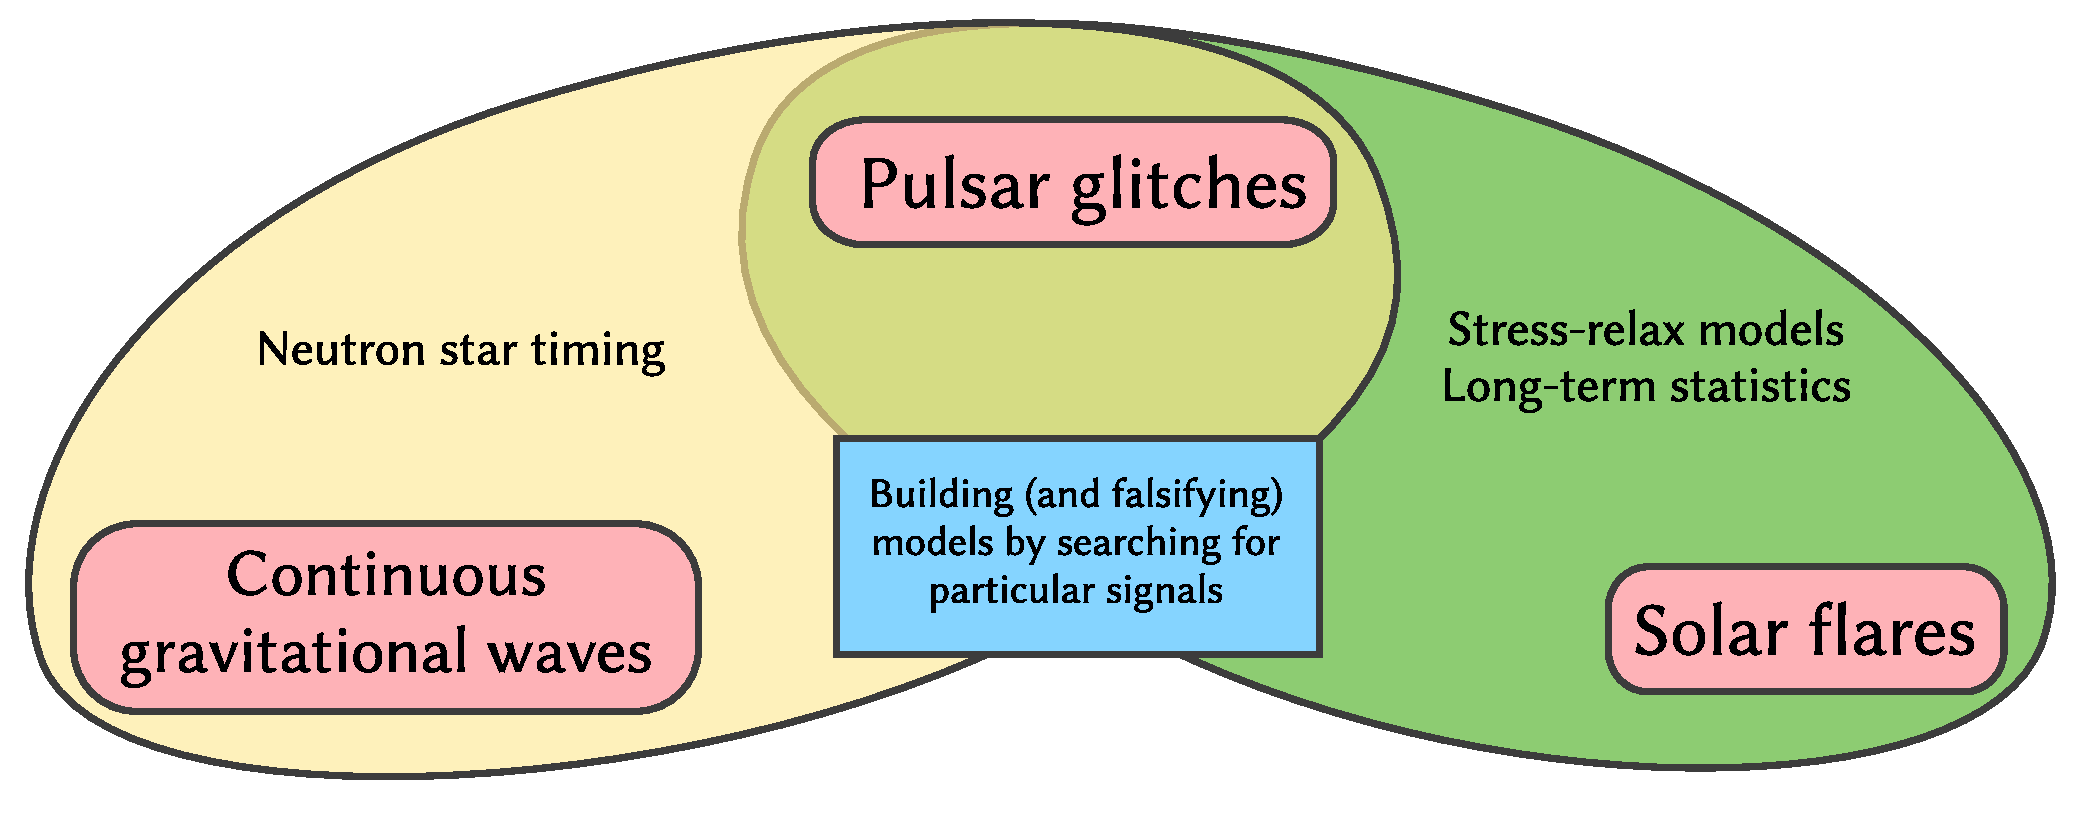
\includegraphics[width=\linewidth]{schematic_v2.pdf}
    \caption{Schematic showing the three major topics of this thesis in red, while the overarching theme that links all the topics is in blue. Pulsar glitches and continuous gravitational waves are connected in yellow by both having to do with neutron star timing; glitches are seen as sudden deviations from a steady timing solution, while a sensitive continuous gravitational wave search is enabled by pulsar timing providing reference ephemerides. A continuous wave detection would result in an independent timing solution. Pulsar glitches and solar flares are connected in green via the underlying mechanism with which they operate, namely that stress builds up steadily over time, and is released suddenly. Long-term sequences of waiting times between events, and event sizes, allow for falsification of these stress-relax models.}
    \label{fig:thesis_schema}
\end{figure}

\section{Observational taxonomy of neutron stars} \label{sec:intro_ns}
A neutron star is the dense remnant of a massive star (with mass $9 \lesssim M / M_\odot \lesssim 25$, where $M_\odot$ is the mass of the Sun), after it has undergone a core collapse supernova \citep{Shapiro1983}. First theorized to exist by \citet{Baade1934}, direct observational evidence came over 30 years later with the discovery of a steadily pulsating radio source by then-PhD candidate Jocelyn Bell-Burnell and her supervisor Antony Hewish \citep{Hewish1968}. This object, the pulsar now known as PSR J1921$+$2153, was quickly designated as a rotating neutron star \citep{Gold1968,Pacini1968}, and many more pulsars were discovered soon after \citep{Pilkington1968,Large1968,Turtle1968,Turtle1968a,Comella1969}.

After 55 years of new discoveries, the variety of neutron stars with differing properties allows us to form a taxonomy broadly divided into two categories:
\begin{itemize}
    \item \textbf{Isolated neutron stars} are seen most commonly as radio pulsars, but are also detected across the electromagnetic spectrum, e.g.~optical, infrared, gamma-ray, and X-ray. Isolated pulsars are typically further classified into two main groups, so-called ``rotation-powered'' and ``magnetars''. The former have spin periods of $0.01 \lesssim P / \textrm{s} \lesssim 10$, and time-derivative of their period of $10^{-16} \lesssim \dot{P} \lesssim 10^{-12}$. The latter are generally slower but spin down faster, with $P \gtrsim 1\,\textrm{s}$ and $\dot{P} \gtrsim 10^{-13}$ \citep{Lyne2012}. Some pulsars do not fit in the above two groups, for example if they only pulse intermittently, so-called ``rotating radio transients'' (RRATs) \citep{Keane2011}. Some isolated neutron stars do not exhibit pulsations at any wavelength, e.g.~central compact objects (CCO, also called supernova remnants), which often have a black-body spectrum peaked in the X-rays \citep{Pavlov2004,Chevalier2005}. We discuss in Section~\ref{sec:intro_timing} how pulsar timing is performed, and the timing irregularities, such as glitches, that are found in the process.
    
    The mechanism generating pulsed radio emission is an unsolved problem in the field (see \citet{Cerutti2017}, \citet{Harding2017} and references therein). A recent critique by \citet{Melrose2021a} dismisses many of the currently favored models; the authors propose an alternative mechanism in \citet{Melrose2021} (see also the work of \citet{Philippov2020}). Whatever the emission mechanism, as the pulsed emission is coherent, the emission region must be small and offset from the rotation axis of the neutron star --- leading to a ``lighthouse effect'' where the emission region periodically enters our line-of-sight. Thermal black-body emission peaked at shorter wavelengths (e.g.~X-ray) is attributed to the residual heat in the neutron star crust which is slowly dissipating after the supernova that formed the object (typically observable for $\sim10^5\,$yr) \citep{Zavlin2009}. 
    
    \item \textbf{Binary neutron stars} are also sometimes seen as radio pulsars, but are more often detected due to their X-ray emission (so-called ``X-ray binaries''). This emission is thought to arise due to accretion from their companion star forming hot-spots on the surface of the star. The mass of the companion further categorizes X-ray binaries as either low-mass (LMXB, companion mass $M_\textrm{c} \lesssim M_\odot$), intermediate mass (IMXB, companion mass $1 \lesssim M_\textrm{c} / M_\odot \lesssim 10$), or high mass (HMXB, companion mass $M_\textrm{c} \gtrsim 10 M_\odot$) \citep{Psaltis2006}. Typically, the accretion in LMXBs is fed from an accretion disk, while in HMXBs it is fed via stellar winds from the companion \citep{Bondi1944,Karino2019}. 
    
    Some binary neutron stars are observed to have millisecond periods, and are thus called millisecond pulsars (MSPs). MSPs usually have quite small period derivatives, $\dot{P} \lesssim 10^{-18}$, compared to standard rotation-powered pulsars. However, most X-ray binaries are not seen as pulsars, for example neither Scorpius X-1 nor Cygnus X-2 have detectable pulsations \citep{Galaudage2022}. A small fraction of compact (projected semi-major axis $a_0 \lesssim 2\,$lt-s) LMXBs intermittently go into outburst, where the X-ray flux is enhanced by roughly two orders of magnitude for days to months (depending on the object and outburst) \citep{DiSalvo2022}. During these periods of outburst pulsations are sometimes detectable, which puts these objects in a separate class of ``accreting millisecond X-ray pulsars'' (AMXPs). We return to AMXPs in Section~\ref{sec:intro_amxp}.
    
    The small spin period of MSPs is explained via a recycling mechanism, in which the magnetocentrifugal torque exerted by accretion spins up the neutron star \citep{Ghosh1977,Ghosh1979a,Tauris2012}. Some MSPs are not seen in binaries, which is explained via a few pathways: either the neutron star could have fully ablated their companion (as seen in progress in so-called ``black widow'' pulsars), or dynamical effects resulting from a dense stellar environment could have disrupted the binary.
\end{itemize}

The above distinctions are driven by observations, and there are many systems that straddle the border between the outlined categories, or even move between categories \citep{Kaspi2010}. For example, transitional millisecond pulsars, also known as redbacks, are sometimes observed as accretion-powered X-ray binaries, and then as rotation-powered radio pulsars \citep{Campana2018}. Magnetars and CCOs are likely newly born neutron stars with strong birth magnetic fields \citep{Woods2006}. The orientation of the emission region with respect to our line-of-sight could explain why some objects pulsate and some do not.

\begin{figure}
    \centering
    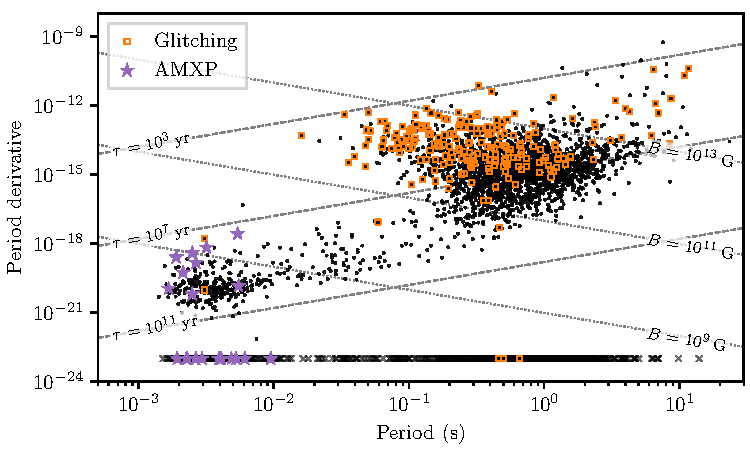
\includegraphics[width=0.85\linewidth]{ppdot.pdf}
    \caption{Period $P$ and period derivative $\dot{P}$ diagram for over 3300 objects retrieved from the ATNF Pulsar Catalog. Black crosses sitting at the bottom of the figure are pulsars which do not have a recorded $\dot{P}$. Orange boxes indicate pulsars with at least one recorded glitch, and are the objects of interest for Chapters~\ref{chap:acorr}--\ref{chap:hda} of this thesis. Purple stars mark the known AMXPs, which are the objects of interest for Chapter~\ref{chap:amxp} of this thesis. Dotted and dashed lines show lines of constant magnetic field at the poles and characteristic age respectively. }
    \label{fig:intro_ppdot}
\end{figure}
    
Typically, the pulsar population is visualized in a $P-\dot{P}$ diagram, such as Figure~\ref{fig:intro_ppdot}. Each black dot is a pulsar recorded in the Australian Telescope National Facility (ATNF) Pulsar Catalog \citep{Manchester2005}\footnote{Accessed via \url{https://www.atnf.csiro.au/research/pulsar/psrcat/}.}. Black crosses near the abscissa mark pulsars without a recorded period derivative, constituting nearly 23\% of pulsars in the catalog. Objects marked with an orange square indicate that at least one glitch is recorded for that pulsar (see Section~\ref{sec:intro_struc} for more on glitches). AMXPs are marked with a purple star. Lines of constant characteristic age $\tau$ and magnetic field strength at the poles $B$ are shown as dashed and dotted lines respectively. These two quantities are calculated by modeling the pulsar as a simple rotating magnetic dipole \citep{Pacini1967,Pacini1968,Gunn1969} for which the electromagnetic power emitted is
\begin{equation}
\dot{E}_\textrm{dipole} = \frac{-4\pi^4B^2R^6\sin^2\alpha}{3c^3 P^4}\,,\label{eq:dipole_power}
\end{equation}
where $R$ is the neutron star radius, $\alpha$ is the angle between the rotation and magnetic axes, and $c$ is the speed of light. Combining Equation~\eqref{eq:dipole_power} with the rate of change of the rotational kinetic energy 
\begin{equation}
\dot{E}_\textrm{rot.} = \frac{-4\pi^2I \dot{P}}{P^3}\,,\label{eq:rot_power} 
\end{equation}
where $I$ is the moment of inertia of the neutron star, gives
\begin{equation}
B \approx 3.2 \times 10^{19}\,\textrm{G}\, \left(\frac{I}{10^{45}\,\textrm{g\,cm}^2}\right)^{1/2} \left(\frac{R}{10^6\,\textrm{cm}}\right)^{-3} \sqrt{\dot{P} P}\,,\label{eq:magstrength}
\end{equation}
where we have included fiducial values for $I$ and $R$, and set $\sin\alpha=1$. The characteristic age is calculated by assuming that none of the parameters in Equation~\eqref{eq:magstrength} vary in time from birth at $t=0$ to the current age $\tau$ (besides $P$), and integrating $\dot{P} \propto 1/P$ to find
\begin{equation}
\tau = \frac{P^2 - P^2_0}{2 \dot{P}P} \approx \frac{P}{2\dot{P}}\,,\label{eq:char_age}
\end{equation}
where we assume the birth period $P_0 \ll P$. 

Pulsars are almost certainly not perfectly rotating magnetic dipoles in a vacuum, and thus the above calculations are true only to zeroth order. They do apply remarkably well in some individual circumstances, e.g.~the Crab pulsar (PSR J0537+2200) which is associated with a supernova remnant that was observed in 1054 AD by contemporary Chinese astronomers \citep{Mayall1939}. The current measurements of $P \approx 0.033\,$s and $\dot{P}\approx 4.2\times10^{-13}$ \citep{Lyne2015} give $\tau \approx 1258\,$yr, only off from the true age by $\sim 300\,$yr. The power implied by Equation~\eqref{eq:rot_power} of $\dot{E}_\textrm{rot.} \approx -4.5\times10^{38}\,$erg\,s$^{-1}$ (assuming $I = 10^{45}\,\textrm{g\,cm}^2$) is comparable to the total energy requirements of the Crab nebula, $5\times10^{38}\,\textrm{erg\,s}^{-1}$ \citep{Hester2008}, implying that the energy lost due to rotation is likely absorbed and re-emitted by the nebula surrounding the pulsar.

\section{Pulsar timing} \label{sec:intro_timing}
There is a multi-stage process to ``time'' a pulsar, i.e.~model and track the rotation over time. Most pulsars are not bright enough to resolve individual pulses, so the first stage is ``folding'' $5-30\,$minutes (depending on the pulsar and observatory) of radio intensity time-series data, i.e.~averaging the data modulo the fiducial rotation period of the pulsar \citep{Lorimer2004}. 

In the second stage the folded data is correlated with a pulse shape template to generate a highly precise reference time for the observation, known as a time of arrival (TOA). The TOA for an observation is defined as the time at which we have zero rotational phase, i.e.~$\phi = 0$. A correction is applied to each TOA to subtract the effect of the motion of the observatory around the solar system barycentre (SSB).

In the third and final stage, a model is fit to a series of TOAs to model the phase as a function of time, noting that $\phi(t)$ must be an integer at each TOA. Traditionally, the phase is modelled as a simple Taylor series 
\begin{equation}
    \phi(t) = \phi(t_0) + \nu (t - t_0) + \frac{\dot{\nu}}{2}\left(t - t_0\right)^2 + \frac{\ddot{\nu}}{6} \left(t - t_0\right)^3 + \delta\phi(t)\,,\label{eq:taylor_phase}
\end{equation}
where $t_0$ is an arbitrary reference time, $\nu = \frac{\td\phi}{\td t}\big|_{t=t_0}$, $\dot{\nu} = \frac{\td^2\phi}{\td t^2}\big|_{t=t_0}$, and $\ddot{\nu} = \frac{\td^3\phi}{\td t^3}\big|_{t=t_0}$. The phase residuals $\delta\phi(t)$ are studied for features of non-Gaussian noise, i.e.~signatures that the Taylor series phase model does not adequately explain the data. Software such as {\sc{tempo2}} \citep{Hobbs2006,Edwards2006} performs an iterated weighted-least-squares \citep{Press2007} procedure to calculate the values of various pulsar parameters which minimize $|\delta\phi(t)|^2$. These parameters include but are not limited to: $\nu$, $\dot{\nu}$, $\ddot{\nu}$, right ascension and declination (henceforth RA and Dec. respectively), proper motion, and any relevant binary orbital elements.

Recent advances in modelling stochastic variations in $\delta\phi(t)$ have led to extensions to {\sc{tempo2}}, such as the software {\sc{temponest}} \citep{Lentati2014} and the Hidden Markov Model (HMM) tracking described by \citet{Melatos2020hmm}. We discuss these approaches further in Sections~\ref{sec:intro_tn} and \ref{sec:intro_gd} respectively.

\subsection{Timing noise} \label{sec:intro_tn}
The residuals $\delta\phi(t)$ often have a time-correlated stochastic structure that is not expected from measurement errors alone. The structure is also not attributable to incorrectly modelled (deterministic) pulsar parameters such as position or proper motion on the sky \citep{Cordes1980,Shannon2010}. The power spectrum of such residuals is red, with a mixture of random walks in $\nu$ and $\dot{\nu}$, alongside discrete jumps in $\phi$. These residuals are typically called ``timing noise'' \citep{Cordes1985,DAlessandro1995}. Timing noise makes precision timing experiments such as pulsar timing arrays (PTAs) difficult \citep{Perera2019,Arzoumanian2020,Chen2021,Goncharov2021a}. The Bayesian inference software {\sc{temponest}} performs parameter inference on not just the deterministic pulsar parameters, but also estimates the amplitude and spectral index of the power spectral density (PSD) of the residuals by simultaneously modelling a red noise process and the deterministic phase evolution in the frequency domain.   

However, while such an approach can model the aggregate statistical properties of the residuals, it explicitly does not model the observed instantiation of the stochastic process. That is, it does not fit the specific time-ordered sequence of residuals to a particular stochastic process, only their time-averaged statistical properties. On the other hand, one may treat $\phi$, $\nu$, and potentially $\dot{\nu}$, as hidden random variables that are estimated via a hidden Markov model (HMM) \citep{Melatos2020hmm}. We summarize the work of \citet{Melatos2020hmm} in the context of glitch detection in the following subsection, and discuss the mathematical formulation of a HMM in the context of searches for gravitational waves in Section~\ref{sec:intro_cw}.

The mechanism causing timing noise is uncertain. What follows is a non-exhaustive list of the various mechanisms posited in the literature:
\begin{enumerate*}
\item free precession \citep{Stairs2000,Brook2013,Kerr2016},
\item undetected debris or planetary companions \citep{Cordes2008,Kerr2015},
\item unmodelled pulse shape changes \citep{Brook2016,Shannon2016},
\item magnetospheric state switching \citep{Kramer2006,Lyne2010},
\item superposition of small rotational glitches \citep{Cheng1987b,Melatos2008},
\item superfluid turbulence \citep{Greenstein1970,Link2012,Melatos2014},
\item variations in external torques \citep{Cordes1981,Cheng1987a}, or
\item variations in the coupling between internal components and the crust \citep{Jones1990}.
\end{enumerate*}

In some contexts, including continuous gravitational wave searches (discussed in more detail in Section~\ref{sec:intro_cw}), timing noise is referred to as ``spin-wandering'' \citep{Bildsten1998,Leaci2015,Suvorova2016,Mukherjee2018}. Spin-wandering is typically, but not always, attributed to stochastic variations in the mass accretion rate $\dot{M}$. We remind the reader that only binary systems will have appreciable accretion; we must appeal to an alternative mechanism to explain spin-wandering in isolated pulsars. Coincident measurements of the instantaneous spin frequency of a pulsar from both a continuous gravitational wave detection and electromagnetic observations would allow estimates of various coupling parameters between the crust (to which the electromagnetic frequency is bound) and core (to which the gravitational wave frequency may be bound) \citep{Meyers2021,Meyers2021a}. The degree of spin-wandering in Scorpius X-1 is estimated by \citet{Mukherjee2018} to limit the coherence time for a continuous gravitational wave search to $\lesssim 10\,$d. Spin-wandering has not been estimated quantitatively in other accreting systems, although recent advances in the state-space formulation of the problem could enable these estimates in the future \citep{Melatos2023}.

\subsection{Glitch detection} \label{sec:intro_gd}
A sudden discontinuity in the gradient of the phase residuals points to the occurrence of a rotational glitch. For example, if a glitch involves only a jump in spin frequency, the magnitude of the phase residuals will show a linear increase with time, while a change in the spin frequency time derivative would result in parabolic phase residuals. We discuss the broad phenomenology of glitches further in Section~\ref{sec:glitch_phenom}. Traditionally, these phase gradient discontinuities are discovered by eye, and two glitchless phase models, i.e.~Equation~\eqref{eq:taylor_phase}, are fit to TOAs before and after the glitch epoch to define the parameters of the glitch. Both timing noise and long, irregular gaps between TOAs can lead to imprecise or degenerate estimates of glitch parameters \citep{Lyne1996, Dunn2021}. 

Recent advances in Bayesian model selection techniques, i.e.~{\sc{temponest}}, may help, but are not yet mature enough to deploy without human supervision \citep{Lower2020}. An automated pipeline that fits phase residuals within a sliding window, and flags deviations from a polynomial regression, is implemented at the Ooty Radio Telescope \citep{Singha2021a}. The HMM-based method outlined by \citet{Melatos2020hmm} simultaneously models the secular and stochastic behavior of the phase. It determines if a glitch is present in the data by comparing the Bayesian evidence for models that do and do not include a glitch. Due to the computational efficiency of the method, and its automated nature, it is possible to quantitatively assess the upper limit of the smallest detectable glitch, at a given confidence level. For the set of 282 pulsars timed in the UTMOST \citep{Jankowski2019} pulsar timing programme the mean upper limit on the glitch size, as a fraction of the spin frequency, is $1.9\times 10^{-8}$, at 90\% confidence. Historic datasets for the Crab and Vela pulsars were analyzed by \citet{Espinoza2014} and \citet{Espinoza2021} respectively, who found that there exists a minimum glitch size in both pulsars. However, this analysis uses a semi-automated technique, for which the discriminating power between timing noise and glitch is unclear.

\section{Neutron star structure} \label{sec:intro_struc}
A supernova explosion will release some fraction of the original star's mass as heat, light, and via a mass outflow. However, much (1--2$M_\odot$) will collapse into a small radius (9--14\,km) and form a neutron star \citep{Shapiro1983}. The possible values of mass and radius for a neutron star are highly dependent on the so-called ``equation of state'' of matter at extreme densities. The equation of state gives the pressure-density relation, allowing one to solve the equations of hydrostatic equilibrium for mass and radius, along with other physical parameters. The behavior of matter under extreme pressures and densities cannot be studied in terrestrial laboratories, however theoretical nuclear physics studies produce tabulated repositories of plausible equations of state \citep{Ishizuka2015,Typel2015}. 

Recent measurements from the Neutron Star Interior Composition Explorer (NICER) X-ray telescope have constrained both the mass and radius for two millisecond pulsars, PSR J0030$+$0451 \citep{Riley2019a,Miller2019a}, and PSR J0740$+$6620 \citep{Riley2021,Miller2021}. Combining these measurements with constraints derived from gravitational wave data of the coalescence of two neutron stars in GW170817 and GW190425 places observations limits on the equation of state \citep{gw170817eos,Raaijmakers2019,Raaijmakers2021,Pang2021}.

Almost all equations of state lead to a layered structure for a neutron star. The outermost layer is a crystalline crust of iron, nickel, and other metals. As one descends deeper into the ``outer crust'' the pressure increases, and inverse beta decay increases the fraction of neutrons. Once the density is larger than $\rho_{\rm drip} \approx 4\times10^{11}\,$g\,cm$^{-3}$, neutrons begin to ``drip'' out of nuclei, which may condense into a superfluid phase \citep{Chamel2008}. In this ``inner crust'' the nuclei form clusters or defects, to which superfluid vortices may pin, a scenario we discuss further in Section~\ref{sec:glitch_trigger}. The nuclei at the bottom of the inner crust, are sometimes referred to as ``nuclear pasta'' \citep{Ravenhall1983,Watanabe2000,Horowitz2015} due to the variety of shapes and structures displayed in proton density isosurfaces in three-dimensional molecular dynamics simulations. Eventually, there is a transition to a region where a superfluid neutron fluid, and a (potentially superconducting) proton-electron plasma, are co-threading \citep{Shapiro1983,Chamel2008}. This region is called the ``outer core''. Below this we arrive at the inner core, where the dominant physics is much more uncertain, but a condensate of deconfined quarks are one possibility \citep{Alford2003}. 

Observational evidence for the superfluid nature of (at least) the outer core comes from the cooling rate of Cassiopeia A \citep{Heinke2010,Shternin2011,Page2011,Wijngaarden2019}. Note, however, that \citet{Posselt2013,Posselt2018} question whether this evidence is biased by the model used to screen noise artifacts from the Chandra X-ray detectors. Glitches provide independent evidence for superfluidity, as explained further in Section~\ref{sec:intro_glitch}. 

\section{Pulsar glitches} \label{sec:intro_glitch}
As discussed in Section~\ref{sec:intro_gd}, glitches are abrupt changes in the spin frequency, and sometimes frequency derivative, of the pulsar. We discuss the broad phenomenology of glitches in Section~\ref{sec:glitch_phenom}, and move on to the physical models that may explain these events in Section~\ref{sec:glitch_trigger}.

\subsection{Phenomenology and statistics} \label{sec:glitch_phenom}
Not all glitches share the same observational characteristics. For example, while the vast majority of recorded glitches involve an increase in the spin frequency (i.e.~$\Delta \nu > 0$), some glitches in magnetars and accreting systems have $\Delta \nu < 0$ \citep{Ray2019a,Younes2020}. While glitches in accreting systems appear to have similar properties to glitches seen in rotation-powered pulsars \citep{Howitt2022}, we do not discuss them further in this thesis. Glitches in magnetars are also not discussed further; they are occasionally accompanied by changes in the pulse shape, hinting that they may be due to a reconfiguration of the magnetic field, rather than any of the mechanisms discussed in Section~\ref{sec:glitch_trigger} \citep{Dib2008,Dib2014,Garcia2015,Mastrano2015}. Most standard spin-down glitches in rotation-powered pulsars do not change the pulse or emission profile \citep{Espinoza2011,Lyne2012}.

The time-scale over which the change in spin frequency occurs (``rise time'') has never been resolved. The most stringent constraint is that it occurs in less than 12.6\,s, at 90\% confidence, for a glitch from the Vela pulsar in 2016 \citep{Palfreyman2018,Ashton2019}. The Vela pulsar is the only glitching pulsar that is constantly monitored, and is bright enough to allow measurements of individual pulses. These properties allowed detailed analysis of the pulse timing immediately before and after the aforementioned glitch, revealing evidence for an ``overshoot'' (``undershoot'') of the spin frequency after (before) the glitch \citep{Ashton2019}. Regardless of whether there is an overshoot, an exponential decay of the spin frequency is often seen, on timescales ranging from seconds to months after the glitch \citep{Yu2013,Ashton2019}. This decay is not always ``complete'', i.e.~in many glitches there remains a permanent increase in both the spin frequency and/or the time derivative thereof \citep{Hobbs2010,Espinoza2011,Dang2020}. Interpretations of these features with respect to possible physical models is presented in Section~\ref{sec:glitch_trigger}.

As discussed in Section~\ref{sec:intro_gd}, the detection of glitches has historically been performed via visual inspection of timing residuals. As such, the completeness of historical catalogs is not well established. In this context a ``complete'' catalog would include all glitches that have occurred in each pulsar down to a selected size. Completeness is hindered by infrequent observations of many pulsars, and by the minimum detectable glitch size. It is not possible to differentiate whether one large or many smaller glitches occur between two observation epochs \citep{Janssen2006,Yu2017b}. Small glitches, with $\Delta \nu / \nu \lesssim 10^{-9}$, may also be hard to distinguish from timing noise, or so-called ``micro-glitches'' \citep{Janssen2006,Chukwude2010}. \citet{Howitt2020} estimates that roughly 100--200 glitches are missing from glitch catalogs by comparing the rate at which new glitching pulsars are detected, and the rate at which the total number of glitches in the catalog grows, ascribing the shortfall as due to insufficient monitoring of known glitching pulsars.

\begin{table}
    \centering
    \caption{Pulsar name, number of recorded glitches $N$, best-fitting waiting time PDF $p(\Delta t)$, size PDF $p(\Delta \nu / \nu)$, forward cross-correlation $\rho_+$, backward cross-correlation $\rho_-$, waiting time autocorrelation $\rho_{\Delta t}$, and size autocorrelation $\rho_{\Delta \nu / \nu}$ for the eight pulsars with $N \geq 10$. The distribution that fits the waiting time and size PDFs best is determined via the AICc. The 95\% confidence intervals for the Spearman cross-correlation coefficients are calculated via Equation~\eqref{eq:ac_rhoci}. The top four pulsars are ``Poisson-like'', while the bottom four are ``quasiperiodic'', see the text for details. Abbreviations are E, PL, LN, and G for exponential, power-law, log-normal and Gaussian respectively.
      \label{tab:glitch_stats}}
    \def\arraystretch{1.8}%
    \resizebox{\textwidth}{!}{%
    \begin{NiceTabular}{l r l l c c c c}
    \toprule
    Name (J2000) & $N$ & $p(\Delta t)$ & $p(\Delta \nu/\nu)$ & $\rho_+$ & $\rho_-$ & $\rho_{\Delta t}$ & $\rho_{\Delta \nu / \nu}$ \\
    \midrule
    PSR J1740$-$3015 & 36 & LN/E & PL & $0.29^{+0.29}_{-0.35}$ & $-0.11^{+0.34}_{-0.32}$ & $0.17^{+0.31}_{-0.35}$ & $0.02^{+0.33}_{-0.34}$ \\
    PSR J0534$+$2200 & 29 & E/LN & PL & $0.10^{+0.36}_{-0.39}$ & $0.13^{+0.36}_{-0.40}$ & $0.19^{+0.35}_{-0.41}$ & $-0.35^{+0.40}_{-0.30}$ \\
    PSR J0631$+$1036 & 17 & E & PL & $0.21^{+0.44}_{-0.54}$ & $-0.19^{+0.54}_{-0.44}$ & $-0.20^{+0.56}_{-0.45}$ & $0.32^{+0.40}_{-0.56}$ \\
    PSR J1413$-$6141 & 14 & PL & E/LN & $0.82^{+0.14}_{-0.50}$ & $-0.31^{+0.63}_{-0.44}$ & $0.01^{+0.57}_{-0.58}$ & $-0.27^{+0.62}_{-0.45}$ \\
    \midrule
    PSR J0537$-$6910 & 53 & G/LN & G & $0.91^{+0.05}_{-0.10}$ & $-0.21^{+0.29}_{-0.25}$ & $-0.13^{+0.29}_{-0.27}$ & $-0.23^{+0.28}_{-0.25}$ \\
    PSR J1341$-$6220 & 33 & LN & LN & $0.62^{+0.20}_{-0.34}$ & $-0.13^{+0.36}_{-0.33}$ & $-0.00^{+0.35}_{-0.35}$ & $-0.08^{+0.36}_{-0.34}$ \\
    PSR J0835$-$4510 & 24 & G & G & $0.19^{+0.37}_{-0.44}$ & $0.19^{+0.37}_{-0.44}$ & $-0.29^{+0.46}_{-0.36}$ & $-0.29^{+0.45}_{-0.35}$ \\
    PSR J1801$-$2304 & 15 & LN/G & E/LN & $0.71^{+0.21}_{-0.56}$ & $-0.29^{+0.60}_{-0.43}$ & $-0.02^{+0.56}_{-0.55}$ & $-0.13^{+0.57}_{-0.49}$ \\
    \bottomrule
    \end{NiceTabular}
    }
\end{table}

As of 2023 March 21 there are 670 glitches from 208 pulsars recorded in the Jodrell Bank Centre for Astrophysics online catalog\footnote{Accessible via \url{http://www.jb.man.ac.uk/pulsar/glitches.html} \citep{Espinoza2011,Basu2022}.}. While much can be learnt from aggregated statistics \citep{Lyne2000a,Espinoza2011,Yu2013,Fuentes2017,Ashton2017,Eya2019,Basu2022}, in what follows we focus on the pulsars that have glitched the most, to enable a disaggregation of the data. Only eight pulsars have more than 10 recorded glitches. The names of these pulsars and the number of recorded glitches, $N$, are listed in the first two columns of Table~\ref{tab:glitch_stats}. Given a set of $N$ events, we construct a set of $N-1$ waiting times\footnote{Due to a 3-yr (5-yr) gap in monitoring between 1979 and 1982 (2012 and 2017) the waiting time between the fourth and fifth (45-th and 46-th) glitch is not included in the analysis for PSR J0534+2200 (PSR J0537$-$6910) \citep{Espinoza2014,Ho2020}.} $\Delta t$, i.e.~the set of differences between consecutive glitch epochs. 

In the third and fourth columns of Table~\ref{tab:glitch_stats} we list the probability density function (PDF) that fits best the set of waiting times, and the fractional glitch sizes, $\Delta \nu / \nu$, respectively. These best-fitting distributions are determined via the corrected Akaike Information Criterion (AICc) \citep{Akaike1974,Hurvich1989}. The AICc computes the relative evidence of the data being described by one model out of a set of models, while correcting for the bias introduced by the models potentially having a different number of parameters. The AICc value of a model is calculated as
\begin{equation}
   \textrm{AICc} / 2 = k - \ln\left(\hat{\mathcal{L}}\right) + \frac{k^2 + k}{N - k - 1}\,,
\end{equation}
where $k$ is the number of model parameters, $N$ is the number of data points that contribute to $\hat{\mathcal{L}}$, the likelihood of the data given the model, maximized over the model parameters. The model with the smallest AICc value minimizes the information lost in having a model that does not perfectly describe the data. For Table~\ref{tab:glitch_stats} the possible models we compare between are an exponential, a Gaussian, a power-law, and a log-normal (E, G, PL, and LN in Table~\ref{tab:glitch_stats} respectively). When the relative probability between the top two models is within 50\% we list both, separated with a slash\footnote{Whether a given model fits the data ``well'' is a subtle point, especially with few data points. The AICc is a reasonable tool, among many, which can quantitatively compare plausible phenomenological models \citep{Gelman2013}.}. 

Waiting time distributions are best described with an exponential or log-normal for PSR J0534+2200, PSR J0631+1036, PSR J1341$-$6220, and PSR J1740$-$3015. They are best described with a Gaussian or log-normal for PSR J0537$-$6910, PSR J0835$-$4510, and PSR J1801$-$2304. PSR J1413$-$6141 has its waiting time PDF best described with a power law. Size distributions are best described by a power law for PSR J0534+2200, PSR J0631+1036, and PSR J1740$-$3015. They are best described by an exponential or log-normal for PSR J1341$-$6220, PSR J1413$-$6141, and PSR J1801$-$2304. Both PSR J0537$-$6910 and PSR J0835$-$4510 have size PDFs best described with a Gaussian. These results are consistent with previous analyses of glitches from individual pulsars \citep{Melatos2008,Fuentes2017,Howitt2018,Fuentes2019}. Typically, glitching pulsars are separated into two distinct groups: ``Poisson-like'' with exponentially distributed waiting times and power-law distributed sizes, or ``quasiperiodic'' with unimodal (i.e.~Gaussian or log-normal) waiting times and sizes \citep{Melatos2008,Howitt2018}. We find that some pulsars, namely PSR J0534$+$2200, PSR J0631$+$1036, and PSR J1740$-$3015, can be adequately described as Poisson-like. Some are quasiperiodic, namely PSR J0537$-$ 6910, PSR J0835$-$4510, PSR J1341$-$6220, and PSR J1801$-$2304. One pulsar, PSR J1413$-$6141 does not cleanly fall into either group. We caution that with such small sample sizes, it may be the case that neither the demarcation into these two groupings nor the assignations above will persist in the future, as more glitches are observed from these and other pulsars.

The cross-correlation between the glitch size and the following (preceding) waiting time is denoted as the forward (backward) cross-correlation $\rho_+$ ($\rho_-$), and is listed in the fifth (sixth) column of Table~\ref{tab:glitch_stats}. The forward cross-correlations are consistent with zero, at the 95\% confidence level, for PSR J0534+2200, PSR J0631+1036, PSR J0835$-$4510, PSR J1740$-$3015, while the other four pulsars have $\rho_+$ greater than zero. That PSR J0537$-$6910 has a strong forward cross-correlation is well-known in the literature, allowing confident prediction of the time until the next glitch \citep{Middleditch2006,Ferdman2018,Antonopoulou2018,Ho2020}. As \citet{Fuentes2019} noted, while some pulsars have a forward cross-correlation that is consistent with zero at the 95\% confidence level, it would be an unlikely coincidence that we would measure $\rho_+ > 0$ in all pulsars just by chance, assuming the null hypothesis of $\rho_+ = 0$. No pulsar has a backward cross-correlation that is different from zero, at the 95\% confidence level.

The autocorrelation between subsequent waiting times $\rho_{\Delta t}$ (sizes $\rho_{\Delta \nu / \nu}$) is listed in the seventh (eighth) column of Table~\ref{tab:glitch_stats}. They are all consistent with zero, at the 95\% confidence level. 

We return to what long-term statistical measures of waiting time and size PDFs, cross-correlations, and autocorrelations can tell us about the physics of pulsar glitches in Chapters~\ref{chap:acorr}--\ref{chap:hda}.

\subsection{Glitch trigger mechanisms} \label{sec:glitch_trigger}
The mechanism causing pulsar glitches is uncertain. Since the discovery of glitches shortly after the discovery of the first pulsar, models have proliferated. In this subsection we review the mechanisms that remain popular in the literature to this day, summarizing the reviews of \citet{Haskell2015,Antonopoulou2022,Antonelli2022,Zhou2022}. 

As discussed in Section~\ref{sec:intro_struc} the interior of a neutron star is likely to contain both a charged plasma (predominantly electrons and protons), as well as a superfluid component (composed of neutrons). The charged plasma will couple tightly to the crust via the electromagnetic interactions, however a superfluid is irrotational in the bulk. The circulation of a superfluid is carried by quantised vortices, the areal density of which corresponds to a local rotation rate of the superfluid \citep{Onsager1949,Migdal1959}. These vortices are regions with zero superfluid density. However, they act as quasiparticles which exert an effective drag force that couples the superfluid and normal components of the fluid on long timescales, due to the scattering of electrons off the vortex cores \citep{Hall1956, Mendell1991}.

A lag between the rotation rate of the normal and superfluid components gives rise to a hydrodynamic Magnus force on the vortices, pushing them radially outwards \citep{Glampedakis2011}. If vortices can flow without restriction an equilibrium will quickly be reached, where the time derivative of the angular speed of the superfluid and normal components is equal. However, vortices are likely ``pinned'' in at least some regions. In the inner crust, lattice defects or nuclei clusters could create energetically favorable locations for vortices \citep{Anderson1975,Alpar1977,Epstein1988,Link1991,Pizzochero1997,Donati2006,Avogadro2007,Link2009a,Seveso2016a}. The pinning potential in each site will likely vary due to the balance between the self-energy required to bend a vortex, and the interaction strength of the vortex and pinning site, as well as the structure of the lattice nearby \citep{Link2022}. In the core, vortices could pin to superconducting flux tubes \citep{Migdal1959,Ruderman1998,Glampedakis2011,Gugercinoglu2014}. Whatever the mechanism, pinning will frustrate the free motion of vortices, leading to an increasing Magnus force over time, as the lag between the fluid components grows. 

Differential rotation of fluid components and/or the crust provides a reservoir of angular momentum with which we can explain glitches \citep{Baym1969}. The mechanism by which the angular momentum is transferred is likely the mass transport of $\sim 10^{10-13}$ vortices (the exact number of vortices needed depends on the size of the glitch, among other factors) \citep{Anderson1975,Alpar1984}. What could trigger the simultaneous unpinning of such a large number of vortices? 

\subsubsection{Superfluid vortex avalanches}
As the Magnus force on a vortex is proportional to the lag between the fluid components, the stress will eventually accumulate until it is enough to unpin the vortex from its pinning site. While details of the motion of superfluid vortices is complex \citep{Link2022}, two-dimensional point-vortex simulations \citep{Howitt2020}, as well as full quantum dynamical simulations \citep{Warszawski2011,Warszawski2013,Lonnborn2019} exhibit ``avalanches'', where the unpinning of a small subset of vortices can trigger a mass unpinning event through ``knock-on'' interactions with their neighbors. Such stick--slip cascade dynamics are emblematic of systems in a state of self-organized criticality, which we discuss further in Section~\ref{sec:intro_stress}.

\subsubsection{Crustquakes}
The crystalline crust of a neutron star is naturally oblate when born, due to the balance of gravitational and centrifugal forces. As the neutron star spins down, this balance changes, and so does the shape of the star \citep{Pines1972}. However, while the interior is an incompressible fluid, the crust can support some mechanical strain. This strain will build up over time until failure occurs: a crustquake. \citet{Ruderman1969} proposed that crustquakes would be able to adjust the moment of inertia sufficiently to explain all glitches, however too much strain would need to build up too quickly to explain the glitching history of some pulsars \citep{Baym1971}. For example, large glitches ($\Delta \nu / \nu \sim 10^{-6}$) would release $\sim10^5$\,yrs of built-up strain, however the Vela pulsar (PSR J0835$-$4510) experiences glitches that large every 2--3 years. The superfluid nature of the interior could assist in building crustal strain, via the elastic stress attributable to vortices pinned to the crust \citep{Ruderman1976,Chamel2006}. Molecular dynamics simulations give maximal breaking strains that are large (of order $\sim 0.1$), which would likely not be reached before the vortices unpin naturally \citep{Horowitz2009}. Despite the above concerns, crustquakes remain a viable mechanism to trigger at least some glitches, a rearrangement of the crust would likely adjust the pinning potentials near the fault-line, in which many vortices may sit, leading to a mass unpinning event \citep{Rencoret2021}.

Unrelated to glitches, crustquakes may play an important role in building ``mountains'' (i.e.~mass asymmetries) on the surfaces of some neutron stars, perhaps enabling the generation of continuous gravitational waves \citep{Ushomirsky2000,Gittins2021,Kerin2022}. We return to mountains on neutron stars in Section~\ref{sec:intro_cw}.

\subsubsection{Superfluid instabilities and other possibilities}
The onset of an instability in the fluid flow may also precipitate a mass unpinning of vortices. While superfluid flow is typically considered smooth, the interaction between the superfluid and normal components could lead to, for example, a Kelvin-Helmoltz \citep{Mastrano2005} or two-stream instability \citep{Andersson2003,Andersson2004}. The excitation of an instability may create a vortex tangle, i.e.~a disruption of the vortex array, which reduces the coupling between the crust and the superfluid \citep{Peralta2006}. The exact mechanism with which superfluid turbulence triggers a glitch is unclear, but it is likely an important ingredient in understanding glitch recoveries \citep{Andersson2007,Mongiovi2017,Haskell2020}.

Mass unpinning of vortices may also occur through so-called ``vortex creep'', where thermal activation continually unpins vortices, allowing an average vortex current and creating an avenue for collective unpinning without avalanche dynamics \citep{Alpar1984,Melatos2009,Gugercinoglu2014,Gugercinoglu2019}. 

\section{Stress accumulation and relaxation} \label{sec:intro_stress}
In light of the complexities of the mechanisms discussed in Section~\ref{sec:glitch_trigger}, it is helpful to summarize the major, phenomenological commonalities. Glitches are (broadly) unpredictable events that become more likely to occur as stress (e.g.~lag in rotation rate between fluid components) accumulates. The amount of stress released after an event is triggered varies over many orders of magnitude. Unpredictable events of varying sizes are hallmarks of a system in a state of self-organized criticality, but are not unique to such systems \citep{Jensen1998,Watkins2015}. 

The canonical example of a system exhibiting self-organized criticality are the sandpiles of \citet{Bak1987,Bak1988}. This mathematical system describes a grid, upon which grains of sand are dropped at a steady rate. If the local gradient of the sandpile height exceeds a threshold, a toppling event is triggered, reallocating some sand to neighboring grid points. This toppling results in avalanches across all length-scales, the size-invariant statistics thereof are widely studied (e.g. by \citet{Hwa1992,Rosendahl1993,DeMenech2000,Lippiello2010}, among many others). Models with a stochastic driving force (``coherent noise'') also exhibit avalanche-like behavior \citep{Newman1996,Sneppen1997,Melatos2009,Sarlis2012}.

Mathematically modelling the repeated accumulation and depletion of stress in a system is complicated by the ``doubly stochastic'' nature of the process. By doubly stochastic we refer to the fact that both the time between events, and the amount of stress released at each event is a random variable. If one assumes various limits, such as the full depletion of the stress reservoir after each event \citep{Daly2006}, or that an event is only triggered when a stress threshold is reached \citep{Daly2007}, the problem becomes analytically tractable. We call such phenomenological descriptions of stress accumulation and relaxation ``meta-models'', as they typically encompass a broad array of more specific micro-physical models.

In the following Section~\ref{sec:intro_sf} we shift our attention to the phenomenon of solar flares, and describe how current thinking positions flares as arising from a stress-relax process. In Section~\ref{sec:intro_sdp} we introduce the state-dependent Poisson (SDP) process, a mathematical framework for understanding a broad range of stress-relax systems. In this thesis we use the SDP framework, or stress-relax meta-model variants thereof, to help understand pulsar glitches.

\subsection{Solar flares}\label{sec:intro_sf}
Our sun is a main sequence star about halfway through its life, at the end of which it will become a red giant, and then a white dwarf. It is not massive enough to become a neutron star, and thus will never be seen to glitch like a pulsar. However, it does exhibit flares. Solar flares are eruptive emissions of electromagnetic radiation \citep{Fletcher2011,Benz2016}. Flares are often, but not always, emitted from sunspots, active regions with magnetic fields an order of magnitude larger than the rest of the star \citep{Solanki2003}. These magnetic fields are visible via magnetograms \citep{Hale1908}, which show flares often occurring on the boundary between differing magnetic polarity regions. Across these so-called ``neutral lines'' we observe loops, prominences, and arcades of plasma following the field lines. A shift in the footpoints of these features results in an abrupt reconfiguration of the magnetic field, releasing stored magnetic energy \citep{Fletcher2011}. Arcade shearing is not the only possible physical mechanism that involves the release of stored energy, see Table 1 of \citet{Green2018} for more. A key concept in most is that when anti-parallel magnetic field lines become close a magnetic reconnection event occurs, dissipating energy into the surrounding plasma \citep{Anzer1982}. Flare prediction is not possible in general, despite much effort \citep{Wheatland2004,Qahwaji2007,Mason2010,Bobra2015,Barnes2016,Camporeale2019,Thibeault2022}. 

While solar flares exhibit a rich phenomenology across the electromagnetic spectrum, the peak flux $f_{\rm p}$ is typically emitted in the X-ray wavelength \citep{Fletcher2011,Benz2016}. For consistency with historical records, modern flare catalogs encode the peak flux of a flare between 1--8\,\AA\ into flare classes: ``A'', ``B'', ``C'', ``M'', or ``X''. A class A flare has $f_{\rm p} < 10^{-7}\,\textrm{Wm}^{-2}$, a class B flare has $10^{-7} \leq f_{\rm p} / (\textrm{Wm}^{-2}) < 10^{-6}$, a class C flare has $10^{-6} \leq f_{\rm p} / (\textrm{Wm}^{-2}) < 10^{-5}$, a class M flare has $10^{-5} \leq f_{\rm p} / (\textrm{Wm}^{-2}) < 10^{-4}$, and class X flares have $f_{\rm p} \geq 10^{-4}\,\textrm{Wm}^{-2}$. These classes are further subdivided via a subsequent number, such that, for example, a class M7.3 flare has $f_{\rm p} = 7.3\times 10^{-5}\,\textrm{Wm}^{-2}$.

Interpreting the sequences of flares from individual active regions through the lens of stress-relax models enables detailed interrogation of the broad underlying mechanism \citep{Rosner1978,Wheatland1998,Wheatland2000corr,Wheatland2008,Kanazir2010,Hudson2019}. In these models, magnetic energy accumulates secularly, and is released abruptly via flares. The long-term statistical consequences of such a model are somewhat different to the complementary phenomenological description of flares as occurring as a result of an avalanche or self-organized critical system \citep{Lu1991,Lu1993,Lu1995a,Charbonneau2001,Thibeault2022}. In particular, while waiting time and size PDFs may or may not differ between models, the avalanche model predicts no long-term memory, e.g.~no cross-correlations between flare waiting times and sizes. We connect solar flare observations with the machinery of the SDP process in Chapter~\ref{chap:sf}, where we search for these cross-correlations and other tell-tale signs of a stress-relax process that is driven towards a static-in-time threshold before each event.

\subsection{State-dependent Poisson process} \label{sec:intro_sdp} 
We can approach modelling a stress-relax process many ways. For example, cellular automata capture local knock-on effects, and the dynamics therein \citep{Bak1988,Warszawski2008,Kerin2022}. An alternative is to track a globally averaged stress, $X$, as it accumulates gradually between events, and depletes suddenly at events. Early work simplified this approach by either assuming the stress reservoir is depleted at each event \citep{Rosner1978,Daly2006} or that the stress reaching a static-in-time threshold triggers an event \citep{Gaizauskas1987,Daly2007,Hudson2019}. These simplifications naturally result in a prediction of a large backward or forward cross-correlation respectively. In the former case this is because the size of a stress release event is purely determined by the waiting time since the last event (which reset the stress to zero). In the latter case the system must accumulate the stress it lost at the previous event, before the threshold is breached again. Broadly speaking, these cross-correlations are not observed in the natural phenomena these models represent, with a few notable exceptions \citep{Lewin1976,Middleditch2006}.

Mathematically, globally averaged stress-accumulation and release is governed as a function of time $t$ by the stochastic differential equation
\begin{equation}
    \frac{\td X}{\td t} = f(X, t) + g(X, t) + J(X, t)\ , \label{eq:gen_jumpsde}
\end{equation}
where we have separated the stress evolution into three parts. The function $f(X, t)$ is the deterministic driver of stress into the system, i.e.~$f(X, t) \geq 0$. The function $g(X, t)$ models the continuous but stochastic variations in the stress (e.g. Brownian motion), while $J(X, t)$ models the stochastic jumps that occur at epochs $t_1, ..., t_i$, i.e.
\begin{equation}
    J(X, t) = \sum_{i=1}^{N(t)} \Delta X_i[X(t_i^-)] \delta(t - t_i)\ ,
\end{equation}
where $N(t)$ is the number of jumps that have occurred up until time $t$, and $\delta(...)$ corresponds to the Dirac-delta function \citep{Daly2006,Daly2007,Wheatland2009}. The size of each stress-release event $\Delta X[X(t_i^-)]$ typically depends on the stress in the system immediately prior to the event, as otherwise one may have $X < 0$, which is non-physical. 

When do stress-release events occur? For the state-dependent Poisson process, this is governed by the instantaneous rate $\lambda[X(t)]$. The PDF of waiting times drawn from a time-dependent Poisson distribution is \citep{Cox1955}
\begin{equation}
    p(\Delta t\, |\, t) = \lambda(t + \Delta t) \exp \left[-\int_{t'}^{t' + \Delta t}\td t' \lambda(t')\right]\ . \label{eq:gen_tdp_wt}
\end{equation}
Given a prescription for \begin{enumerate*}\item $f(X, t)$, \item $g(X, t)$, \item $\lambda[X(t)]$, and \item a method for picking $\Delta X[X(t_i^-)]$,\end{enumerate*} one may evolve Equation~\eqref{eq:gen_jumpsde} forward in time. As noted by \citet{Wheatland2009,Fulgenzi2017}, directly solving Equation~\eqref{eq:gen_jumpsde} is often intractable, except for a restricted set of choices i)--iv). Instead, one may simulate the system via a Monte Carlo automaton, which iteratively picks waiting times and sizes \citep{Wheatland2009,Fulgenzi2017,Carlin2019quasi}. 

A wide variety of physics is encoded in the choices i)--iv). A simple example is if one has $f(X, t) = f$, and $g(X, t) = 0$ the system accumulates stress deterministically between jumps, and is driven at a constant rate $f$. This is the choice made by \citet{Wheatland2008,Wheatland2009,Fulgenzi2017,Carlin2019quasi,Carlin2019ac,Carlin2021endog,Carlin2023sf}, in both solar flare and pulsar glitch contexts. We explore some of the statistical long-term observables of this ``standard'' configuration of the SDP process in Chapter~\ref{chap:acorr}. We search for signatures of a SDP process underlying solar flares in Chapter~\ref{chap:sf}. 

On the other hand, if $g(X, t) \neq 0$ the stress driver has some stochasticity \citep{Daly2006,Daly2007,Carlin2020bsa}. In Chapter~\ref{chap:bsa} we investigate what a stochastic stress driver implies for the long-term statistical observables of the meta-model, again in the context of pulsar glitches. The choice of iv), i.e.~how event sizes are decided, is another key place where physics is encoded in the model. \citet{Wheatland2009,Fulgenzi2017} both have $\Delta X$ as a random variable, drawn from a power law PDF, as the underlying stress-release mechanism assumes scale-free avalanche dynamics \citep{Jensen1998}. As noted by \citet{Carlin2019quasi} the functional form of this PDF has a large impact on all of the long-term observables, not just the PDF of observed event sizes, due to the coupled nature of the equation of motion. In Chapter~\ref{chap:hda} we specialize the SDP process to a particular choice of iv) which makes $\Delta X$ no longer a random variable, but instead a complex function of the stress-release history. This choice allows for a detailed interrogation of the superfluid vortex avalanche model of pulsar glitches.

% \newpage
\section{Continuous gravitational waves} \label{sec:intro_cw}
We turn our attention now to the final topic of this thesis, a search for continuous gravitational waves from AMXPs. In Section~\ref{sec:intro_gw} we briefly review the necessary background to understand gravitational waves. In Section~\ref{sec:intro_det} we introduce the active ground-based gravitational wave detectors. In Section~\ref{sec:intro_emiss} we discuss plausible emission mechanisms for continuous gravitational waves. In Section~\ref{sec:intro_cwmethod} we discuss the standard signal model, while in Section~\ref{sec:intro_hmm} we discuss how considerations of spin-wandering modify it. Finally, in Section~\ref{sec:intro_amxp} we describe why AMXPs are plausible sources for continuous gravitational waves. 

\subsection{General relativity} \label{sec:intro_gw}
In the weak-field limit, Einstein's field equations of general relativity admit wave-like solutions as perturbations $h_{\mu \nu}$ to a flat spacetime metric. In the transverse-traceless gauge a plane wave travelling in the $z$-direction is given by
\begin{equation}
    h_{\mu \nu}(t, z) = \begin{pmatrix}
        0 & 0 & 0 & 0 \\
        0 & h_+ & h_\times & 0 \\
        0 & h_\times & -h_+ & 0 \\
        0 & 0 & 0 & 0
    \end{pmatrix} \exp \left[i \omega \left(\frac{z}{c} - t\right) \right]\ , \label{eq:planewave}
\end{equation}
where $\omega$ is the gravitational wave angular frequency, $h_+$ is the $+$ polarization amplitude, $h_\times$ is the $\times$ polarization amplitude, and the tensor components of $h_{\mu\nu}$ are given by the matrix elements. The dominant contribution for a non-relativistic source at a distance $D$ is,
\begin{equation}
    h_{\mu \nu} (t, x^i) = -\frac{2 G}{D c^4} \frac{\td^2}{\td t^2} \left[I_{\mu \nu}\left(t - \frac{D}{c}\right)\right]\ , \label{eq:hmunu}
\end{equation}
where $G$ is the gravitational constant, $c$ is the speed of light, and $I_{\mu \nu}$ is the mass quadrupole moment tensor, calculated viz.
\begin{equation}
    I^{\mu \nu} = \int \td^3x T^{00}x^\mu x^\nu\ , \label{eq:massquad}
\end{equation}
where $T^{00}$ is the time-time component of the stress-energy tensor \citep{Schutz2022}. The monopole and dipole contributions to gravitational radiation vanish due to conservation of energy and momentum respectively. A time varying mass-current multipole also generates gravitational waves. Adopting the notation of \citet{Thorne1980}, a mass-current multipole produces a wave with components
\begin{equation}
    h_{\mu \nu} (t, x^i) = \frac{2 G}{D c^4} \sum_{l=2}^{\infty} \sum_{m=-l}^{m=l} \pd{^l S^{lm}(t - D/c)}{t^l} T^{B2,lm}_{\mu \nu}\,, \label{eq:hmunu_current}
\end{equation}
where $S^{lm}$ is the $(l,m)$-th current multiple moment, and $T^{B2,lm}_{\mu \nu}$ are components of the tensor spherical harmonic, not the stress-energy tensor \citep{Mathews1962,Thorne1980}. We return to both time-varying mass quadrupole and mass-current sources in Section~\ref{sec:intro_emiss}.

Equations~\eqref{eq:hmunu} and \eqref{eq:hmunu_current} result in wave amplitudes too small to detect, unless the gravitational wave source is a compact object with a large, rapidly varying moment of inertia or current. We restrict our attention to single sources of gravitational radiation, i.e.~we do not discuss the stochastic gravitational wave background (see \citet{Renzini2022} for a comprehensive review of modern stochastic gravitational wave searches). 

The one confirmed gravitational wave source to date are coalescing binaries composed of black holes or neutron stars, as detected routinely by the LIGO-Virgo-KAGRA Collaboration (LVK) since 2015 \citep{150914obs,gwtc3}, and detected indirectly via orbital shrinkage in pulsar binaries \citep{Weisberg1981}. Other, short-duration ($\lesssim 100\,$s) so-called ``burst'' gravitational wave sources include core-collapse supernovae \citep{Powell2019,Radice2019}, cosmic strings \citep{Vachaspati1985,Sakellariadou1990}, and pulsar glitches \citep{Warszawski2012a,Yim2020,Ho2020a}, but are yet to be detected \citep{o3aburst,o3aburst_string}. In this thesis we do not consider binary coalescence or burst gravitational wave sources further. Rapidly rotating non-axisymmetric neutron stars are a plausible source of continuous gravitational waves, and are discussed further in Sections~\ref{sec:intro_emiss}--\ref{sec:intro_hmm}. 

\subsection{Ground-based gravitational wave detectors} \label{sec:intro_det}
The most sensitive gravitational wave detectors to a broad range of frequencies are laser interferometers \citep{Weiss1972}. Currently, there are five large interferometers around the world: the two LIGO detectors in the United States of America (in Livingston Louisiana, ``L1'', and Hanford Washington, ``H1''), Virgo in Italy, KAGRA in Japan, and GEO 600 in Germany. As the work in Chapter~\ref{chap:amxp} uses only data from the LIGO detectors, we will focus our attention there.

The LIGO detectors are power-recycled Fabry-Pérot Michelson interferometers with 4\,km arms. As a gravitational wave passes through a detector, the length difference $\Delta L(t)$ between the arms varies as a function of time. Measuring the dimensionless strain $h(t) = \Delta L(t) / L$, where $L$ is the arm length, allows one to infer the polarization amplitudes $h_+$ and $h_\times$ of the gravitational wave, given adequate information about the source direction and inclination. The sensitivity of the detectors to a given strain is typically quantified in the frequency domain, by calculating the amplitude spectral density (ASD) $S^{1/2}(f)$ of the noise in units of Hz$^{-1/2}$. Figure~\ref{fig:asds} shows the improvement in the typical ASD for the L1 detector between the fifth Science Run (S5), which ran from November 2005 to September 2007, and the second half of the third Observing Run (O3b), which ran from November 2019 to March 2020. The roughly order-of-magnitude improvement in ASD allows one to detect an order-of-magnitude smaller amplitude gravitational wave, at a fixed signal-to-noise ratio (SNR), when using matched filtering method such as the ones discussed in Section~\ref{sec:intro_cwmethod}.

\begin{figure}
    \centering
    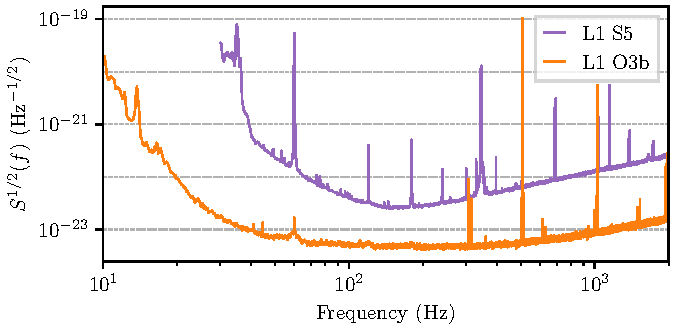
\includegraphics[width=0.8\linewidth]{s5_o3b_asds.pdf}
    \caption{Representative ASDs for the Livingston (L1) LIGO detector in S5 (purple curve) and O3b (orange curve). The ASDs are representative in that they are calculated from $\sim5\,$min of data for a period of time in which the detectors are operating within their modal binary neutron star detection range for that observing run, see \citet{Weinstein2010,o3b_asd} for details.} \label{fig:asds}
\end{figure}

\subsection{Continuous gravitational wave emission mechanisms} \label{sec:intro_emiss}
Continuous gravitational waves are both persistent, with durations $\gtrsim 1\,$yr, and ``quasi-monochromatic''. In this context, quasi-monochromatic corresponds to the frequency of the gravitational wave $f_{\rm GW}$ in the frame of the gravitational wave detector varying by $\lesssim0.01\,$Hz over the course of a year. These small variations in frequency are due to different factors, depending on the source of the continuous gravitational wave, which we explain further in Section~\ref{sec:intro_cwmethod}. The prototypical continuous gravitational wave source is a rapidly rotating non-axisymmetric neutron star, which may or may not be in a binary system. 

There are many physical processes that may lead to the asymmetry of the source. For example ``mountains'' (either on the surface or in the interior of the star) which lead to a time-varying mass quadrupole could be supported via thermoelastic \citep{Baym1971,Ushomirsky2000,Johnson-McDaniel2013}, magnetic \citep{Cutler2002,Mastrano2011,Lasky2013}, or tectonic processes \citep{Middleditch2006,Chugunov2010,Giliberti2022,Kerin2022}. A perpendicular biaxial rotor (e.g.~a rigid star with a mountain symmetrically straddling the equator) will emit GW at a frequency $f_{\rm GW} = 2f_\star$, where $f_\star$ is the underlying neutron star rotation frequency. If the principal axis of the moment of inertia and the rotation axis are offset by a ``wobble'' angle $0 < \theta < \pi / 2$, the system freely precesses and will emit gravitational waves at both $f_\star$ and $2f_\star$, and potentially other harmonics \citep{Zimmermann1979,Zimmermann1980,Jones2002}. 

For the simplest case of a perpendicular biaxial rotor rotating around its $z$ axis, the strain is \citep{JKS98}
\begin{equation}
    h_0 = \frac{4\pi^2 G}{c^4} \frac{\epsilon I_{zz} f_{\rm GW}^2}{D} \, \label{eq:h0_eps}
\end{equation}
where $h_0 \equiv |h_{+ / \times}|$ (if the system is inclined edge-on to the detector), and $\epsilon =  |I_{xx} - I_{yy}| / I_{zz}$.

Oscillation modes in the interior of a neutron star may lead to gravitational wave emission via a time-vary mass-current multipole, see Equation~\eqref{eq:hmunu_current}. Rotation-dominated axial modes (so-called $r$-modes, in analogy to Rossby modes on Earth) are unstable under gravitational wave emission \citep{Andersson1998,Friedman1998,Owen1998}. By unstable, we refer to the mode amplitude growing exponentially with time, due the current moving retrograde in the frame of reference rotating with the neutron star, but prograde in an external frame; thus gravitational radiation removes positive angular momentum from a mode that has negative angular momentum, increases the strength of the current \citep{Friedman1998}. The oscillation mode grows until a saturation amplitude $\alpha$ is reached, when non-linear hydrodynamic and viscous effects damp the growth \citep{Alford2012}. Once the mode saturates, it may be active for years or decades \citep{Arras2003}. The gravitational wave frequency, in the slow-rotation Newtonian limit, is 
\begin{equation}
    f_{\rm GW} = m \left[1 - \frac{2}{l(l+1)}\right] f_\star\ , \label{eq:fgw_rmode}
\end{equation}
where $l$ and $m$ are the standard orders of a multipolar expansion \citep{Papaloizou1978}. The $l=m=2$ mode is most susceptible to the above instability, and is the least likely to be damped by viscous effects \citep{Lindblom1998,Andersson1999}, leading to $f_{\rm GW} = 4f_\star / 3$. Accounting for the impact of rapid rotation, a realistic equation of state, and corrections due to general relativity is complex. These considerations lead to suggestions that searches for gravitational waves from $r$-modes should allow for $1.39 - 0.195 (f_\star / f_{K})^2 \lesssim f_{\rm GW} / f_\star \lesssim 1.57$, where $f_K$ is the Keplerian frequency at which a neutron star breaks up \citep{Idrisy2015,Caride2019}. 

An $r$-mode generates gravitational waves with strain
\begin{equation}
    h_0 = \sqrt{\frac{512 \pi^7}{5}} M R^3 \tilde{J}\, \frac{\alpha f_{\rm GW}^3}{D}\ , \label{eq:h0_alpha}
\end{equation}
where $M$ and $R$ are the mass and radius of the neutron star respectively, and $\tilde{J}$ is an equation-of-state-dependent dimensionless quantity, typically taken as $\tilde{J} \approx 0.0164$ \citep{Owen1998,Owen2010}. 

A pinned superfluid also results in a mass-current quadrupole, leading to a gravitational wave signal similar to that of a precessing star, i.e.~at $f_\star$ and/or $2f_\star$ \citep{Peralta2006,Eysden2008,Bennett2010,Jones2010,Melatos2015}.

\subsection{Standard signal model} \label{sec:intro_cwmethod}
While the many processes discussed in Section~\ref{sec:intro_emiss} are quite different in nature, the signal processing techniques needed to detect a continuous gravitational wave are broadly independent of the generation mechanism \citep{Owen2010,Riles2013a}. In the global Lorentz frame of reference of an observer not moving relative to the center of mass of the neutron star, the phase of the gravitational wave is typically modelled as a Taylor series, as in Equation~\eqref{eq:taylor_phase}. By the time the gravitational wave reaches the detectors on Earth there are modulations to this phase. For concreteness (and simplicity), in what follows we consider a perpendicular biaxial rotor, i.e.~we have $\theta = \pi/2$ and only consider emission at $f_{\rm GW} = 2f_\star$. The data $x(t)$ in a single detector is
\begin{align}
    x(t) &= F_+(t) h_+(t) + F_\times(t) h_\times(t) + n(t)\ ,\label{eq:gw_xoft}
\end{align}
where $F_{+/\times}(t)$ are beam-pattern functions given as equations (10)--(14) in \citet{JKS98}, and $n(t)$ is the time-dependent noise. The beam-pattern functions describe the response of the detector to a given gravitational wave strain. They depend on the orientation, longitude, latitude, and opening angle of the detector, as well as the RA, Dec., and polarization angle $\psi$ of the source (see Figure~1 of \citet{Wette2023} for a visual representation of this angle). The other components of Equation~\eqref{eq:gw_xoft} are given by
\begin{align}
    h_+(t) &= \frac{1}{2} h_0 \left(1 + \cos^2\iota \right) \cos \Phi(t)\ ,\label{eq:hplus} \\
    h_\times(t) &= h_0 \cos\iota \sin \Phi(t)\ , \label{eq:htimes}
\end{align}
where $\iota$ is the inclination angle of the source's total angular momentum vector with respect to our line of sight, and $\Phi(t)$ is given by Equation~\eqref{eq:taylor_phase} with the addition of time-dependent terms to account for the diurnal and annual motions of the Earth. For a source at a given sky location the signal has $5 + s$ unknown parameters: $h_0, \psi, \iota, \Phi_0, f_{\rm GW}, f^{(s)}_{\rm GW}$, where $\psi$ is the polarization angle, $\Phi_0$ is an arbitrary phase offset, $s$ is the number of frequency-derivatives included in Equation~\eqref{eq:taylor_phase}, with $f^{(s)}_{\rm GW}$ denoting the $s$-th time derivative of the frequency. For a source in a binary system there is an additional Doppler modulation, which introduces three additional parameters, the semimajor axis $a$ projected on the sky $a_0 = a \sin \iota$, the orbital period $P$, and an additional phase offset, typically defined at the time of passage through the ascending node $T_{\rm asc}$. Explicitly, the binary orbit introduces a Rømer delay $\Delta_R(t)$, which shifts the time at which a given gravitational wave phase reaches the SSB by 
\begin{equation}
    \Delta_R(t) = a_0 \sin \frac{2\pi(t - T_{\rm asc})}{P}\,, \label{eq:binary_mod}
\end{equation}
see Section 2.2 of \citet{Wette2023} for details. The above assumes circular orbits for both the Earth, and the object in its binary system. It is possible to account for non-circular orbits in general \citep{Leaci2015}, however LMXBs typically have negligible measured eccentricity \citep{Bhattacharyya2022}.

One approach to search for the above signal is to construct the optimal maximum-likelihood matched filter called the $\mf$-statistic \citep{JKS98}. The matched filter analytically maximizes the log-likelihood of the data over a subset of the (typically unknown \emph{a priori}) parameters, i.e.~$h_0$, $\psi$, $\iota$, and $\Phi_0$. Due to the numerical efficiency of the fast Fourier transform, the $\mf$-statistic is typically computed in the frequency domain \citep{JKS98,Prix2009a}.

A $\mf$-statistic-based search typically iterates over a template bank of the remaining unknown parameters, recording which parameter combinations result in detection statistic values that exceed a threshold. The requisite spacing of the templates is determined by the ``metric'' of the detection statistic, i.e.~one calculates the maximum distance with which templates can be placed without diminishing the SNR overmuch \citep{Leaci2015}. Precise knowledge of the unknown parameters reduces the volume of this search space, and thus increases the probability of detection at a fixed probability of false alarm, due to a reduced effective trials factor.

While the $\mf$-statistic can account for the additional Doppler modulation due to binary motion \citep{LAL2018}, there are numerous alternatives or augmentations which trade off between numerical and detection efficiencies. By numerical efficiency we refer to the ability of a search algorithm to save and re-use intermediate data products, reducing the total computational cost of searching a template bank. By detection efficiency we refer to the ability of a search algorithm to detect a given signal strength in noise, typically estimated empirically through a campaign of software injections and recoveries. 

A circular binary orbit causes the gravitational wave phase to vary harmonically, c.f.~Equation \eqref{eq:binary_mod}. If unaccounted for, this harmonic modulation creates so-called ``orbital sidebands'' \citep{Messenger2007,Sammut2014}, i.e. periodic peaks in the power spectrum with spacing $2\pi/P$. The $\mathcal{C}$-statistic incoherently sums the power dispersed into these sidebands \citep{Sammut2014}. The $\mj$-statistic uses a Jacobi-Anger expansion of the phase to construct a coherent matched filter, allowing for increased detection efficiency at the expense of requiring knowledge of (or a search over) $T_{\rm asc}$ \citep{Suvorova2017}. See Section 3 of \citet{Suvorova2017} for mathematical and implementation details of the $\mj$-statistic.

To demonstrate the breadth of signal processing techniques applied to search for continuous gravitational wave signals from neutron stars in binary orbits, we present a non-exhaustive list of search algorithms and/or detection statistics in Table~\ref{tab:binarycw_overview}. For detailed, modern reviews, see \citet{Piccinni2022,Riles2023,Wette2023}. 

\begin{table}
    \centering
    \caption{Non-exhaustive list of algorithms and/or detection statistics used to search for continuous gravitational wave signals from neutron stars in binary orbits. ``TD'' refers to a search performed in the time (rather than frequency) domain. ``Sco X-1'' refers to Scorpius X-1, a LMXB discussed further in Section~\ref{sec:intro_amxp}. Directed searches have a fixed sky position (i.e.~the target is known from electromagnetic observations), but search a wide frequency band. Targeted searches have a fixed sky position, and fix the gravitational wave phase evolution to an exact harmonic of the electromagnetically observed phase evolution. Blind searches are not targeting a known system, but instead search the whole sky and a wide frequency band. Narrowband searches have a fixed sky position, but search a narrow frequency band around harmonics of the electromagnetically observed spin frequency. O1, O2, and O3 refer to Observing Runs 1, 2, and 3 respectively of the LVK. S5 and S6 refer to Science Runs 5 and 6 respectively of the LIGO detectors. Only searches using the latest data searched (fourth column) are listed in the sixth column.
     \label{tab:binarycw_overview}}
    \def\arraystretch{1.8}%
    \resizebox{\textwidth}{!}{%
    \begin{NiceTabular}{l p{2cm} l p{2cm} p{2.2cm} p{2.2cm}}
    \toprule
    Algorithm & Target(s) & Search type & Latest data searched & Method reference(s) & Search reference(s) \\
    \midrule
    5n-vector       & Sco X-1 & Directed & O2 & \citep{Astone2012,Singhal2019} & \citep{Singhal2019} \\
                    & Known MSPs & Targeted & O3 & \citep{Astone2012} & \citep{o3known} \\
    BinarySkyHough  & Unknown MSPs & Blind & O3 & \citep{Covas2019} & \citep{o3abinaryallsky,Covas2022} \\
    $\mathcal{C}$-statistic & Sco X-1 & Directed & O1 & \citep{Sammut2014} & \citep{o1vitsco}\tabularnote{Uses a hidden Markov model framework to track spin-wandering, see Section~\ref{sec:intro_hmm}.} \\
    CrossCorr       & Sco X-1 & Directed & O3 & \citep{Dhurandhar2008,Whelan2015} & \citep{o3crosscorSco,Whelan2023}\\
    $\mj$-statistic & Sco X-1 & Directed & O3 & \citep{Suvorova2017} & \citep{o3vitsco}\tabularnote{Uses a hidden Markov model framework to track spin-wandering, see Section~\ref{sec:intro_hmm}.} \\
                    & Known MSP & Directed & O3 & \citep{Suvorova2017} & \citep{Vargas2023}\tabularnote{Uses a hidden Markov model framework to track spin-wandering, see Section~\ref{sec:intro_hmm}.} \\
                    & AMXPs & Narrowband & O3 & \citep{Suvorova2017} & \citep{o3amxp}\tabularnote{Uses a hidden Markov model framework to track spin-wandering, see Section~\ref{sec:intro_hmm}.} \\
    TD $\mf$/$\mathcal{G}$-statistic & Known MSPs & Targeted & O3 & \citep{JKS98,Jaranowski2010} & \citep{o3known} \\
    TD Bayesian     & Known MSPs & Targeted & O3 & \citep{Pitkin2017} & \citep{o3known} \\ 
    TwoSpect        & Sco X-1 & Directed & S6 & \citep{twoSpectInit} & \citep{s6twoSpectScoXTE} \\
                    & AMXP & Narrowband & S6 & \citep{twoSpectInit} & \citep{s6twoSpectScoXTE} \\
                    & Unknown MSPs & Blind & S6 & \citep{twoSpectInit} & \citep{s6twospectAllsky} \\
    \bottomrule
    \end{NiceTabular}
    }
\end{table}

Despite differing approaches to the numerical and computational challenges of a continuous gravitational wave search, the algorithms and/or detection statistics in Table~\ref{tab:binarycw_overview} have the same inherent signal model. They assume the signal phase varies deterministically, according to Equation~\eqref{eq:taylor_phase}, plus the requisite Doppler corrections. Coherent searches track the phase over the entire data span $T_{\rm obs} \sim 1\,$yr (for a typical observing run of the LVK), but are prohibitively expensive unless many of the unknown spin parameters, including $f_{\rm GW}$ and $\dot{f}_{\rm GW}$ are fixed at values inferred via electromagnetic observations.  However, if the template bank is large, a semi-coherent technique which splits the data span into $N_T$ segments of length $T_{\rm drift}$ is employed. Semi-coherent pipelines do not require phase continuity between blocks. Often, semi-coherent pipelines follow up candidates above the initial search threshold by increasing the coherence time $T_{\rm drift}$, which will increase the SNR if the signal conforms to the deterministic phase model discussed above \citep{Whelan2015,Keitel:2021xeq}. 

For continuous gravitational wave searches targeting known pulsars, i.e.~targets with an electromagnetically measured $f_\star$, so-called ``targeted'' or ``narrowband'' searches are typically conducted. A targeted search assumes a strict signal model that the $\Phi(t)$ in Equations~\eqref{eq:hplus} and \eqref{eq:htimes} is an exact harmonic of the electromagnetically measured phase, i.e.~$f_{\rm GW}$ (and time-derivatives thereof) are assumed to be known exactly \citep{o3aknown,o3known}. On the other hand, a narrowband search allows a slight mismatch between $f_\star$ ($\dot{f}_\star$) and the harmonics at which $f_{\rm GW}$ ($\dot{f}_{\rm GW}$) may exist. The degree of allowed mismatch varies, but recent searches allow for $1 - \delta < f_{\rm GW} / (2 f_\star) < 1 + \delta$, with $\delta \sim 10^{-3}$ \citep{o3aknown,o3narrowband}. The rationale for allowing such a mismatch is that the gravitationally emitting mass or current quadrupole may not co-rotate exactly with the electromagnetically emitting component of the star. For example, there may exist differential rotation between the crust and core, as discussed in Sections~\ref{sec:intro_struc} and \ref{sec:glitch_trigger}.

\subsection{Hidden Markov Models and wandering signals} \label{sec:intro_hmm}
Timing noise, or spin-wandering as it is often called in continuous gravitational wave contexts, is ubiquitous in pulsars, as discussed in Section~\ref{sec:intro_tn}. The effect that spin wandering has on the standard signal model discussed in Section~\ref{sec:intro_cwmethod} depends on both the continuous gravitational wave emission mechanism, and the mechanism underlying spin wandering. Most emission mechanisms predict $f_{\rm GW} \propto f_\star$, as discussed in Section~\ref{sec:intro_emiss}, so if $f_\star$ fluctuates stochastically, so will $f_{\rm GW}$. This stochastic fluctuation limits the coherence time over which the deterministic signal model discussed above is valid.

One method of incorporating a stochastically fluctuating frequency into the signal model is by treating $f_{\rm GW}$ as a hidden random variable. This hidden random variable is observable through noisy measurements, i.e.~matched filters with a deterministic signal model applied to segments of data $T_{\rm drift}$ in length. To search for such a hidden random variable, a standard signal processing technique is to frame the problem in terms of a hidden Markov model (HMM) \citep{Baum1966}. Concretely, a HMM describes a Markovian random process that moves between a finite set of discrete states $\{q_1,...,q_{N_Q}\}$ over a finite set of discrete time steps $\{t_1,...,t_{N_T}\}$. The possible trajectories of the process are determined probabilistically via the transition matrix $A_{q_i q_j}$, which gives the probability of moving to state $q_i$ from state $q_j$. This transition matrix is combined at each timestep with the emission probability $L_{o_i q_j}$, which gives the probability of observing the noisy measurement $o_i$ if the process is in the state $q_j$. The probability of a trajectory through the set of states $Q = \{q(t_1),...,q(t_{N_T})\}$ given a set of observations $O = \{o(t_1),...,o(t_{N_T})\}$ is
\begin{equation}
    \textrm{Pr}(Q\,|\,O) = \Pi_{q(t_1)} \prod_{i=2}^{i=N_T} L_{o(t_i)q(t_i)} A_{q(t_i)q(t_{i-1})}\ , \label{eq:prqo}
\end{equation}
where $\Pi_{q(t_1)}$ is the prior probability of starting in each state. The Viterbi algorithm \citep{Viterbi1967} efficiently solves the problem of finding the most probable trajectory $Q^*$ through the state--time trellis, given a set of observations and a prescribed transition matrix. It does so in a dynamic, recursive manner; at every timestep the algorithm only retains most-likely trajectories ending in each of the $N_Q$ states. Once the final timestep is reached, the most probable trajectory is reconstructed via backtracking. See equations~(14)--(19) of \citet{Suvorova2016} for a pseudocode implementation of the Viterbi algorithm. We show a toy illustration of the Viterbi algorithm recovering an injected signal in noise in Figure~\ref{fig:viterbi_ill}.
 
\begin{figure}
    \centering
    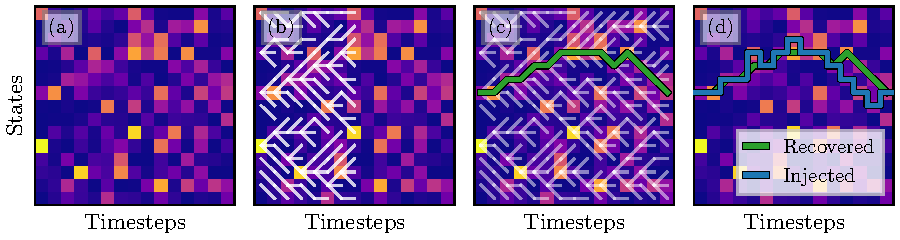
\includegraphics[width=\linewidth]{viterbi_toy.pdf}
    \caption{Illustration demonstrating the Viterbi algorithm finding a wandering signal in noise. The color for each state and time represents the likelihood $L_{o_i q_j}$, with purple and yellow corresponding to low and high relative $L_{o_i q_j}$ respectively. In panel (a) we have injected a wandering signal into noise. In panel (b) we see the Viterbi algorithm dynamically pruning the possible trajectories of the signal in white. In panel (c) we highlight the maximum \emph{a posteriori} trajectory in green, i.e.~the trajectory that maximizes Equation~\eqref{eq:prqo}. Finally, in panel (d) we reveal the trajectory of the injected signal in blue, and show that the trajectory recovered by the Viterbi algorithm overlaps with it.} \label{fig:viterbi_ill}
\end{figure}

Mapping the physics of spin-wandering onto a HMM-based search for continuous gravitational waves requires us to choose: i) a method of estimating $L_{o_i q_j}$ for a given time chunk of length, ii) the duration $T_{\rm drift}$ over which $f_{\rm GW}$ stays within one frequency bin, and iii) the transition matrix $A_{q_i q_j}$ \citep{Suvorova2016}. For i) we assign the hidden discrete states of the HMM to $f_{\rm GW}$, and thus use a frequency-domain estimator for $L_{o_i q_j}$. Typically, for searches targeting isolated sources the $\mf$-statistic is used \citep{Sun2019,Millhouse2020,Beniwal2021,Jones2021,o3aSNR}, while the $\mj$-statistic is used for targets in binary systems \citep{o2vitsco,o3amxp,o3vitsco}, however other choices exist \citep{o1vitsco,Bayley2019,Melatos2021}. For ii) and iii), the most common choice is to assume that spin-wandering amounts to an unbiased random walk in $f_{\rm GW}$. One way to approximate an unbiased random walk in a HMM is to choose 
\begin{equation}
    A_{q_{i+1} q_i} = A_{q_{i} q_i} = A_{q_{i-1} q_i} = \frac{1}{3}\ ,\label{eq:aqiqj}
\end{equation}
with all other elements zero, such that at each timestep the process may move one state up or down, or stay in the same state, with each option having equal probability. We limit $T_{\rm drift}$ such that $f_{\rm GW}$ moves at most one frequency bin $\Delta f$ over $T_{\rm drift}$. We set $\Delta f = 1 / (2T_{\rm drift})$, i.e.~we over-sample the Nyquist frequency by a factor of two. For LMXBs, fluctuations in $f_\star$ are inferred from X-ray flux fluctuations \citep{Bildsten1998}, which then map to fluctuations in $f_{\rm GW}$ via the mechanisms discussed in Section~\ref{sec:intro_emiss}. X-ray flux fluctuations indicate auto-correlation time-scales of order $\sim10\,$days \citep{Mukherjee2018}, informing our choice of $T_{\rm drift}$. 

\subsection{Accreting millisecond X-ray pulsars} \label{sec:intro_amxp}
First discovered in 1998, AMXPs provide concrete evidence for the so-called ``recycling scenario'' of radio millisecond pulsars. In this scenario, a no-longer-pulsating neutron star (having spun down into the so-called ``death valley'', the bottom-right corner of the $P$--$\dot{P}$ diagram, see Figure~\ref{fig:intro_ppdot} \citep{Chen1993}) has a stellar-mass binary companion. The companion eventually overflows its Roche lobe due to standard binary evolution, creating an accretion disk around the neutron star. The matter in this accretion disk is funneled onto the magnetic poles of the neutron star, providing a torque that can spin it up, ``reviving'' the neutron star as a millisecond pulsar \citep{Radhakrishnan1982,Alpar1982}. 

There is an abrupt cut-off in the spin frequency distribution of millisecond pulsars, with none observed spinning faster than $f_\star \approx 716\,$Hz \citep{Hessels2006}. Millisecond oscillations in the tails of thermonuclear X-ray bursts also provide evidence for an upper limit in spin frequency for neutron stars that do not persistently pulsate \citep{Chakrabarty2003}. The fastest spinning AMXP has $f_\star \approx 599\,$Hz \citep{Patruno0029}. The distribution of spin frequencies for AMXPs is statistically consistent with a uniform distribution between 100 and 600\,Hz, as assessed via a Kolmogorov-Smirnov test (p-value of 0.91). The frequency at which a neutron star is disrupted via centrifugal effects is uncertain, however most estimates put it at higher than 1\,kHz \citep{Cook1994}. This implies that either the torque due to accretion must switch off at a certain frequency, or there is an opposing, balancing torque that stops the neutron star in these systems from spinning up to the break-up frequency. 

The microphysical details of accretion onto a magnetized neutron star are complex, so we summarize only the pertinent details here, and refer the interested reader to modern reviews in \citet{Patruno2021,DiSalvo2022}, and references therein. Adopting the simplistic model of steady accretion from a geometrically thin disk onto a star with dipolar magnetic field with magnetic moment $\mu$, the radius $r_m$ at which the freely-falling gas has comparable kinetic and magnetic energy density in the magnetosphere is 
\begin{align}
    r_m &= \xi\, \left(\frac{\mu^4}{2 G M \dot{M}^2}\right)^{1/7}\ , \\
    &\approx 18\,\textrm{km}\, \left(\frac{\xi}{0.5}\right)\, \left(\frac{\mu}{10^{26}\,\textrm{G\,cm}^3}\right)^{4/7} \left(\frac{\dot{M}}{10^{-10}\,M_\odot\textrm{yr}^{-1}}\right)^{-2/7} \left(\frac{M}{1.4\,M_\odot}\right)^{-1/7}\ , \label{eq:magnetoradius}
\end{align} 
where $\dot{M}$ is the mass accretion rate at the inner boundary of the disk, and $\xi \approx 0.3-1.0$ corrects for the non-spherical geometry, non-dipolar magnetic field, and more, see \citet{DAngelo2010} for details. Without the correction factor $\xi$, $r_m$ is more commonly known as the Alfvén radius, $r_A$. The distance $r_m$ is where the gas transfers angular momentum to the neutron star, applying a torque. This torque spins up the star, if we have $r_m < r_{\rm co}$, where $r_{\rm co}$ is the radius at which the gas is co-rotating in a Keplerian orbit, with the same angular frequency as the surface of the star, i.e.
\begin{align}
    r_{\rm co} &= \left(\frac{GM}{4\pi^2 f_\star^2}\right)^{1/3} \\
    &\approx 18\,\textrm{km}\,\left(\frac{M}{1.4\,M_\odot}\right)^{1/3} \left(\frac{f_\star}{900\,\textrm{Hz}}\right)^{-2/3}\ . \label{eq:comovradius}
\end{align}
On the other hand, if $r_m > r_{\rm co}$, the accretion torque will have the opposite sign, i.e.~it will spin down the star. This implies that, under the assumptions of the above simple model, accretion will only spin up the neutron star until $r_m \sim r_{\rm co}$, which occurs at $f_\star \approx 9\times10^2\,$Hz for the fiducial values inserted into Equations~\eqref{eq:magnetoradius} and \eqref{eq:comovradius} above \citep{Ghosh1979a,White1997}. This equilibrium frequency depends on $\mu$ and $\dot{M}$, which can in principle be estimated from X-ray data \citep{Melatos2023}. In the above argument we have obviated the complexity of the magnetic field interacting not just with the inner boundary, but the entire accretion disk \citep{Wang1987,Rappaport2004}, among other considerations. 

An alternative explanation for the lack of observed spin frequencies above 716\,Hz is that gravitational wave emission balances the torque provided via accretion \citep{Bildsten1998}. The torque produced by gravitational waves $N_{\rm GW}$ depends on the degree of asymmetry, as well as the rotation frequency, viz. \citep{Bildsten1998}
\begin{equation}
    N_{\rm GW} = -\frac{32G \epsilon^2 I_{zz} (4\pi f_\star)^5}{5c^5 }\ , \label{eq:gwtorque}
\end{equation}
where we have assumed the simple ``mountain'' emission mechanism discussed in Section~\ref{sec:intro_emiss}. If we also assume the simple model for the accretion torque above (i.e.~neglecting the additional torque induced by the interaction of the magnetic field with the accretion disk), we have \citep{Ghosh1979a}
\begin{equation}
N_{\rm acc} = \dot{M} \sqrt{GM r_m}\,. \label{eq:acctorque}
\end{equation}
When we let Equation~\eqref{eq:gwtorque} balance Equation~\eqref{eq:acctorque}, we rearrange to find
\begin{align}
    f_\star \approx&~ 767\,\textrm{Hz}\ \left(\frac{M}{1.4\,M_\odot}\right)^{-3/70} 
    \left(\frac{I_{zz}}{10^{45}\,\textrm{g\,cm}^2}\right)^{1/5} 
    \left(\frac{\xi}{0.5}\right)^{1/10}
    \left(\frac{\mu}{10^{26}\,\textrm{G\,cm}^3}\right)^{4/70} \nonumber \\
    &\times\ \left(\frac{\epsilon}{10^{-7}}\right)^{-2/5}
    \left(\frac{\dot{M}}{10^{-10}\,M_\odot\textrm{yr}^{-1}}\right)^{-3/35}\,, \label{eq:fstar_equil}
\end{align}
where we have inserted Equation~\eqref{eq:magnetoradius} for $r_m$. That is, for reasonable values of $\epsilon \sim 10^{-7}$ \citep{Ushomirsky2000,Melatos2005,Haskell2006}, the gravitational wave back-reaction torque will balance the torque from accretion at a spin frequency for which $r_m < r_{\rm co}$, i.e.~before the magnetospheric radius increases to the point where accretion begins to spin down the star.  

Typically, $\dot{M}$ is assumed to be proportional to the X-ray flux $F_X$, as the maximum possible accretion luminosity is $L=(GM\dot{M})/R$, and $F_X = L/(4\pi D^2)$. Thus, at fixed $f_{\rm GW}$ and $\epsilon$, sources with the highest $F_X$ will produce the largest $h_0$ (see Equation~\eqref{eq:h0_eps}) \citep{Wagoner1984,Bildsten1998}. This torque-balance argument motivates continuous gravitational wave searches for Scorpius X-1, the brightest extra-solar X-ray source in the sky, and is a LMXB which likely hosts a neutron star \citep{s6twoSpectScoXTE,o1crosscorSco,o1vitsco,o2vitsco,Zhang2021,o3vitsco,o3crosscorSco,Whelan2023}. No detection of continuous gravitational wave emission is claimed. There are multiple reasons why searches for continuous gravitational waves from this target are challenging: 
\begin{enumerate*}
    \item no pulsations have been seen, thus the rotation frequency of the neutron star is unknown \citep{Galaudage2022};
    \item relatedly, the binary orbital elements are poorly constrained \citep{Killestein2023}; and
    \item flux variations indicate the timescale of spin-wandering is $T_{\rm drift} \sim 10\,$days \citep{Mukherjee2018}.
\end{enumerate*}
Items i) and ii) require search algorithms iterate through not only the plausible frequency range, but also a large template bank of orbital elements. The impact of item iii) is ameloriated with a HMM-based search method, as introduced in Section~\ref{sec:intro_hmm}, but still limits the chunk of time $T_{\rm drift}$ over which coherent integration is feasible. 

AMXPs are alternative LMXB targets for continuous gravitational wave searches. They are a heterogeneous class of objects, with few features that are shared among all known AMXPs, hence the conditional statements below. For detailed reviews, see \citet{Marino2019,Patruno2021,DiSalvo2022}. Most AMXPs are in a quiescent state most of the time, with no X-ray pulsations visible. The typical X-ray flux in this state is three to four orders of magnitude smaller than that for Scorpius X-1 (c.f.~Table~\ref{tab:exp_ul} and references therein). Sporadically, AMXPs go into ``outburst'', where their X-ray flux is enhanced by roughly two orders of magnitude, and X-ray pulsations are usually detectable. The durations of and waiting times between outburst phases are usually unpredictable, with durations ranging from minutes to months, and some AMXPs going decades between outbursts. The enhanced X-ray flux is interpreted as a temporary increase in the mass accretion rate. Coherent timing, as discussed in Section~\ref{sec:intro_timing}, is performed whenever pulsations are visible. These timing solutions reveal both positive and negative spin-frequency derivatives, which are small in magnitude, typically $\dot{f}_\star \sim \pm 10^{-14}\,$Hz\,s$^{-1}$. There is little concrete evidence of spin-wandering in AMXPs, however timing noise is found in some \citep{Patruno2009a}, and accretion torques are observed to vary on timescales of weeks in others \citep{Campana2018}. By connecting timing solutions from different outbursts, a long-term negative spin-frequency derivative ($\dot{f}_\star \sim -10^{-15\,}$Hz\,s$^{-1}$) is found in some AMXPs \citep{Papitto2011,Riggio2011,Patruno1808}. 

What is the motivation behind searching for continuous gravitational waves from AMXPs specifically? Variable accretion rates, and evidence that these systems are not in spin equilibrium (i.e.~$\dot{f}_\star \neq 0$), limit the direct application of the classic torque-balance argument \citep{Bildsten1998}. However, it is unclear whether the sharp cut-off in spin frequency is adequately explained from accretion theory alone \citep{Chakrabarty2003,Patruno2012a}, especially given transient accretion episodes can spin up AMXPs to higher spin frequency compared to persistent accretors \citep{Bhattacharyya2017}. Active accretion events can plausibly deposit sufficient material to form mountains \citep{Bildsten1998,Cutler2002,Melatos2005,Haskell2017a}, or ring-up $r$-modes \citep{Andersson1999a,Bondarescu2013,Alford2015}. A search in modulations of X-ray spectra tentatively reveals $r$-mode oscillations may exist in some AMXPs \citep{Mahmoodifar2013,Strohmayer2014}. Detection of continuous gravitational waves is likely difficult, given the suspected small strains, and the current sensitivity of the detectors \citep{Watts2008,Haskell2015GW}. However, searches are computationally inexpensive as both the spin frequency and orbital elements of AMXPs are well known from electromagnetic timing solutions provided from X-ray pulsations. The timescale of spin-wandering in AMXPs is not well understood. We use $\tdr=10\,$d for consistency with previous analyses of Scorpius X-1 \citep{Sammut2014, o1vitsco, o2vitsco, o3vitsco}, where the timescale of spin-wandering is constrained via studies of the X-ray flux variability \citep{Mukherjee2018}.

Searches were performed in both S6 \citep{s6twoSpectScoXTE} and O2 LIGO data \citep{Middleton2020} for one and five AMXPs respectively. In Chapter~\ref{chap:amxp} we perform a HMM-based search for continuous gravitational waves from 20 AMXPs using O3 LIGO data. 

\newpage
\section{Thesis outline} \label{sec:intro_outline}
We structure the remainder of the thesis as follows.
\begin{itemize}
    \item Chapter~\ref{chap:acorr} investigates how autocorrelations between glitch waiting times or sizes provide an additional statistical tool for falsifying the SDP process, as the underlying meta-model governing how glitches are triggered. We show that the SDP process cannot currently be falsified in any individual pulsar, but the diversity of statistical classes of glitching pulsars necessitates that the distribution of stress-release sizes must vary pulsar-to-pulsar. This tentatively indicates that different physical mechanisms are triggering glitches in different pulsars.
    \item Chapter~\ref{chap:bsa} introduces a new stress-accumulation and relaxation meta-model wherein the stress accumulates via a biased Brownian random walk, until a stress threshold is reached. The long-term statistical predictions of this meta-model are compared to data, and we show that the model cannot adequately explain the sequences of glitches in all pulsars, unless we are not detecting many small glitches.
    \item In Chapter~\ref{chap:hda} we augment the SDP framework by explicitly tracking the pinning strength of pinning sites that are occupied by vortices over sequences of glitches. Doing so specializes the meta-model to interrogate the superfluid vortex avalanche microphysical model for pulsar glitches. We find that the predictions of such a meta-model are incongruent with the long-term statistical observables from glitching pulsars. 
    \item Chapter~\ref{chap:sf} adapts the SDP framework to the context of solar flares. We search for evidence that solar flares are triggered when an underlying stress variable reaches a static-in-time threshold before each event. We find no strong evidence for this in the historical catalog of flares.
    \item Chapter~\ref{chap:amxp} presents a search for continuous gravitational waves from 20 AMXPs in LIGO O3 data. The search uses a HMM pipeline that explicitly accomodates a stochastically wandering signal model. We find no strong evidence of any signals, and thus set upper limits on the maximum possible asymmetry in these objects.
    \item Chapter~\ref{chap:conc} concludes the thesis with a summary of the above work, and some directions for future work.
\end{itemize}